\documentclass{standalone}
\usepackage{tikz}
\usepackage{ctex,siunitx}
\usepackage{tkz-euclide}
\usepackage{amsmath}
\usetikzlibrary{patterns, calc}
\usetikzlibrary {decorations.pathmorphing, decorations.pathreplacing, decorations.shapes,}
\begin{document}
\small
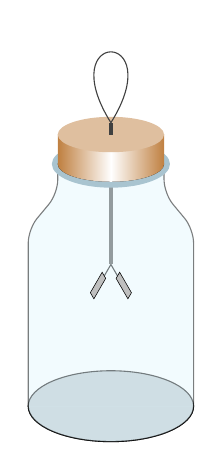
\begin{tikzpicture}[>=latex,scale=1.5]
  % \useasboundingbox(-1,-2)rectangle(8,6);
  \draw[very thick,darkgray](0,0)--(0,1.2);
  \draw(0,0)--(240:0.15)(0,0)--(300:0.15);
  \draw[fill=cyan!10!lightgray](0,-1.2)ellipse(0.7 and 0.3);
  \draw[rounded corners=5pt,fill=cyan!10,opacity=0.5](-0.7,-1.2)--(-0.7,0.3)--(-0.45,0.6)--(-0.45,1.0)--(0.45,1.0)--(0.45,0.6)--(0.7,0.3)--(0.7,-1.2);
  \draw[fill=cyan!10,opacity=0.5](0.7,-1.2)arc(360:180:0.7 and 0.3);
  \fill[cyan!20!lightgray,](0,0.85)ellipse(0.5 and 0.2);
  \fill[left color=brown,right color=brown,middle color=white](0,0.85)ellipse(0.45 and 0.15);
  \fill[left color=brown,right color=brown,middle color=white](0.45,0.85)rectangle(-0.45,1.1);
  \fill[brown!50](0,1.1)ellipse(0.45 and 0.15);
  \draw[very thick,darkgray](0,1.1)--(0,1.2);
  \draw[darkgray](0,1.2)..controls(-0.5,2.0)and(0.5,2.0)..(0,1.2);
  \draw[very thin,fill=lightgray](-0.074,-0.066)--(-0.174,-0.239)--(-0.144,-0.291)--(-0.044,-0.118)--cycle
  (0.074,-0.066)--(0.174,-0.239)--(0.144,-0.291)--(0.044,-0.118)--cycle;
\end{tikzpicture}
\end{document}